
\begin{figure}
    \centering
    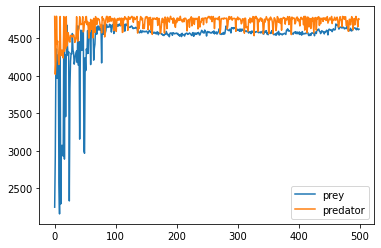
\includegraphics[width=0.5\linewidth]{fig/alive_2_v1.png}
    \caption{Number of alive fish in each generation}
    \label{fig:alive_II_1}
\end{figure}
Figure \ref{fig:alive_II_1} shows the number of alive fish in each generation. Each generation is against the opponents in the hall of fame, meaning their opponents are as good as possible. This is the cause for less generally fish being killed during a predator iteration than a prey one.
\begin{figure}
    \centering
    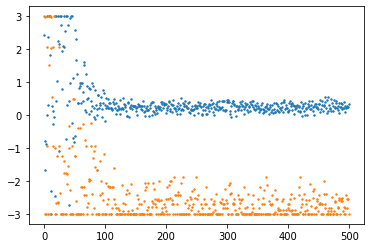
\includegraphics[width=0.5\linewidth]{fig/2-alpha-beta-1.png}
    \caption{$\alpha$ and $\beta$ values tested in each generation}
    \label{fig:a_b_2}
\end{figure}
\begin{figure}
    \centering
    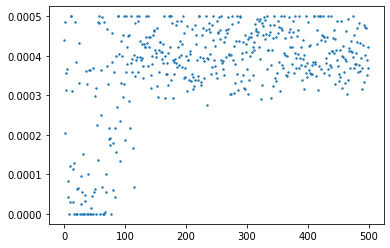
\includegraphics[width=0.5\linewidth]{fig/g_b_2.png}
    \caption{$\delta$ across each generation}
    \label{fig:d_2}
\end{figure}
The parameters tested in some cases cluster together as shown in Figure \ref{fig:a_b_2}, with $\alpha$ staying slightly above 0 and $\beta$ being close to -3. In other cases, such as Figure \ref{fig:d_2}, all values are $>0.0003$ but there is still a large amount of variance within the bounds\footnote{$\delta$ is significantly smaller than the other constants due to the formulae used, and setting the bounds any larger caused it to stay at the minimum value.}. Similar graphs for the predator variables $\gamma_1$ and $\gamma_2$ show no narrowing of valid values at all. The resultant best predators was also very varied.\par
\begin{figure}
    \centering
    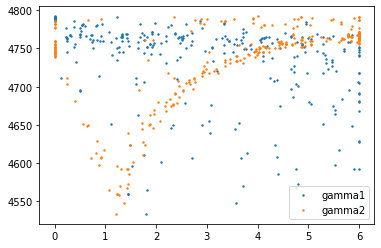
\includegraphics[width=0.5\linewidth]{fig/2_gammas_pred.png}
    \caption{$\gamma_1$ and $\gamma_2$ against number of alive fish (lower means the predator was more successful)}
    \label{fig:2_gammas}
\end{figure}
Figure \ref{fig:2_gammas} was therefore used to select the $\gamma_1, \gamma_2$ and $k$ parameters which were most optimal, as $\gamma_2$ has a clear minimum at just under 1.5. Iterations 351 and 342 were very similar and met this condition of $\gamma_1 = 1.447$, so their values of $\gamma_2$ (1.231) and $k$ (0.4898) were used.\par
The corresponding graphs for the prey variables showed little of interest beyond confirming that $\beta$ should be very close to -3 and $\alpha$ should be $\ge0.25$. As a result, I selected the best performing prey iteration, 461, with $\alpha=0.3885, \beta=-2.700,\gamma=0.3489$ and $\delta=0.00392$.\par
\begin{figure}
    \centering
    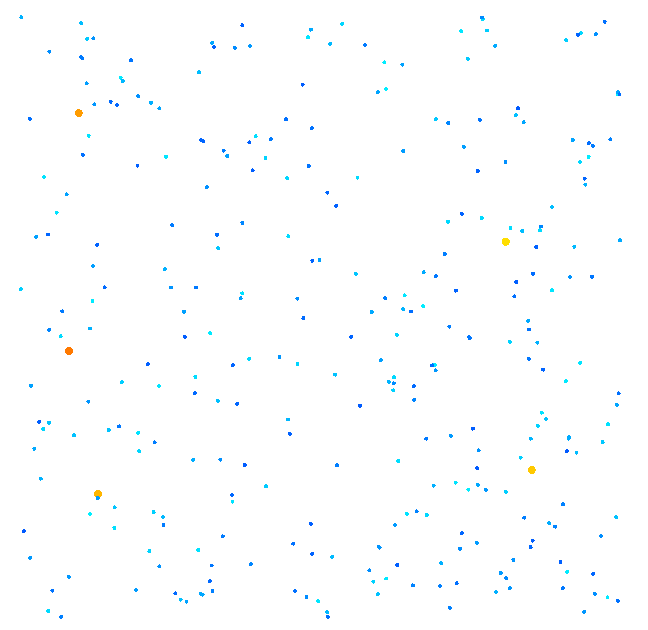
\includegraphics[width=0.5\linewidth]{ii.png}
    \caption{Optimal behaviour for strategy II}
    \label{fig:ii}
\end{figure}
Figure \ref{fig:ii} shows the emergent behaviour with these parameters. As $|\beta|$ is much greater than $|\alpha|$, the main force on prey is to avoid being at the same velocity as their neighbours, resulting in very minimal visible clumps. %insert citation + bioloigical backup here%
\begin{figure}
    \centering
    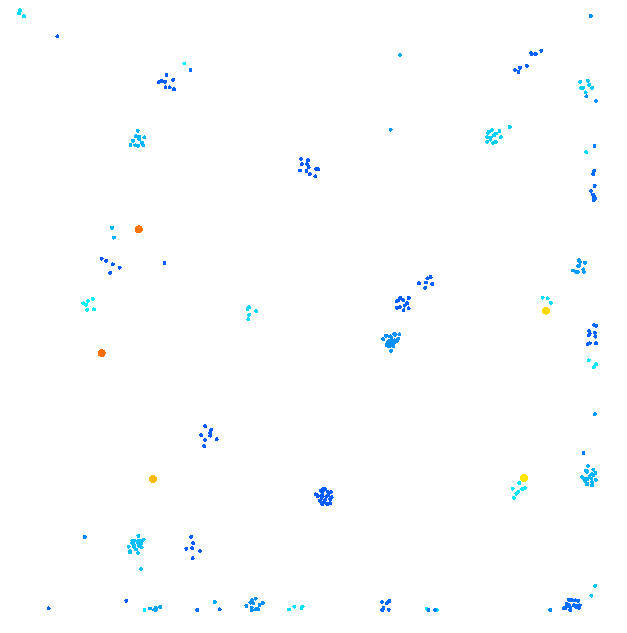
\includegraphics[width=0.5\linewidth]{fig/ii_forced.png}
    \caption{Optimal behaviour for strategy II when schooling is forced}
    \label{fig:placeholder}
\end{figure}
Running the simulation with otherwise the same parameters but setting $\alpha$ and $\beta$ to a minimum of 0.25, forcing schooling, resulted in the average alive fish being closer to 2500 (around 4500 in the previous simulation), and a $\gamma_2$ of zero, suggesting that distance matching is significantly more successful than velocity matching when prey are schooling. $k$ is also very close to 1, showing a preference for smaller schools. $\alpha$ and $\beta$ also remained at the minimum, showing that there is no secondary maximum at which point schooling is preferred.
\begin{figure}
    \centering
    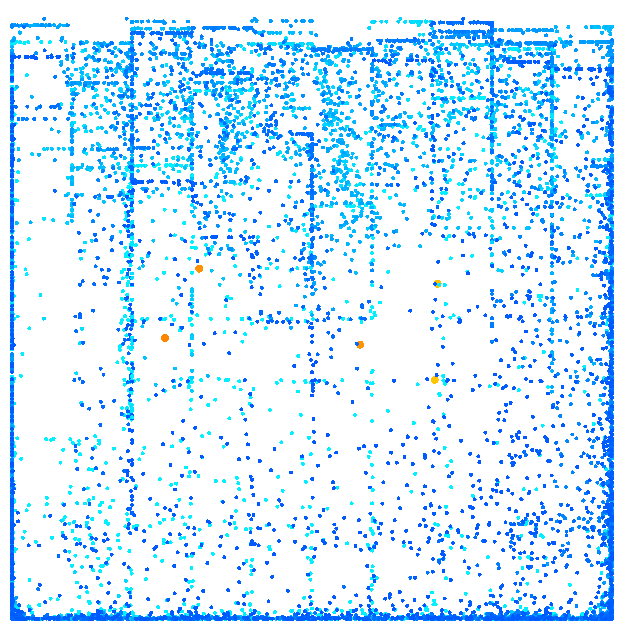
\includegraphics[width=0.5\linewidth]{fig/many_fish.png}
    \caption{10,000 fish with a negative $\gamma$ parameter (attracted to walls), showing obstacles}
    \label{fig:forced walls}
\end{figure}
This simulation was then repeated using the obstacles defined above, set to 1 standard deviation of obstacles is equal to half the tank height. Figure \ref{fig:forced walls} shows how there are now bars from the top of the tank, although they are not shown in the visualisations as it is useful to see the fish behind them.\par
The results of this were generally less well-defined than previous optimisations, likely due to the increased noise from the obstacles. 
The final run of the simulation was using strategy III rather than strategy II, as it is unclear which on cod generally use. \\
[RESULT + VISUALISATION]